\chapter{变系数的 Sasa-Satsuma 方程}
本章我们要研究的方程是变系数的 Sasa-Satsuma 方程,具有如下的项式,
\begin{equation}
  \mathrm{i}u_{t} + \alpha_{1}(t)u_{xx} + \alpha_2(t)|u|^{2}u + \mathrm{i}\left[\alpha_3(t)u_{xxx} + \alpha_{4}(t)(|u|^{2}u)_{x} + \alpha_{5}(t)(|u|^{2})_{x}u + \alpha_{6}(t)u \right] = 0  \label{ss-1}
\end{equation}
其中 $u$ 表示关于变量 $x, t$ 的复函数, $|u|^2$ 表示 $u$ 函数和其共轭函数 $u^*$ 的乘积,方程中各项的系数 $\alpha_1(t) - \alpha_6(t)$ 是关于变量 $t$ 的实函数。

之前已经有关人员对方程 (\ref{ss-1}) 的一些特殊形式进行了相关的研究,例如
\begin{itemize}
  \item 当系数满足 $\alpha_1(t)=\alpha_1, \alpha_2(t)=\alpha_2, \alpha_3(t)=\beta_1, \alpha_4(t)=\beta_2+2\beta_3, \alpha_5(t)=\beta_2+3\beta_3, \alpha_6(t) = 0$ 时,方程 (\ref{ss-1}) 可以被简化为
      \begin{equation}
        \mathrm{i}u_t + \alpha_1 u_{xx} + \alpha_2 |u|^2u + \mathrm{i}\left[\beta_1u_{xxx} + \beta_2|u|^2u_x + \beta_3u(|u|^2)_x\right] = 0,
      \end{equation}
      文献 \cite{ss-46} 给出了该方程的双线性形式和多孤子解。
  \item 当系数满足 $\alpha_1(t)=\dfrac{1}{2}, \alpha_2(t)=1, \alpha_3(t)=\dfrac{1}{6\varepsilon}, \alpha_4(t)=\dfrac{1}{\varepsilon}, \alpha_5(t)=-\dfrac{1}{2\varepsilon}, \alpha_6(t) = 0$ 时,方程 (\ref{ss-1}) 的形式如下
      \begin{equation}
        \mathrm{i}u_t + \frac{1}{2}u_{xx} + u^2u^* + \frac{\mathrm{i}}{6\varepsilon}\left[u_{xxx} + 6uu_xu^* + 3u(uu^*)_x\right] = 0,
      \end{equation}
      文献 \cite{ss-45} 研究了此方程的 Lax 对, Ba\"cklund 变换,单孤子解和无穷守恒律。
  \item 当系数满足 $\alpha_1(t)=\dfrac{1}{2}, \alpha_2(t)=1, \alpha_3(t)=\epsilon, \alpha_4(t)=6\epsilon, \alpha_5(t)=3\epsilon, \alpha_6(t) = 0$ 时,方程 (\ref{ss-1}) 变为
      \begin{equation}
        \mathrm{i}u_t + \frac{1}{2}u_{xx} + |u|^2u + \mathrm{i}\epsilon\left[u_{xxx} + 3(|u|^2)_xu + 6|u|^2u_x \right] = 0,
      \end{equation}
      文献 \cite{ss-40} 使用了达布变换的方式得到了此方程的怪波解。
  \item 当系数满足 $\alpha_1(t)=-1, \alpha_2(t)=-2, \alpha_3(t)=1, \alpha_4(t)=6, \alpha_5(t)=-3, \alpha_6(t) = 0$ 时,方程 (\ref{ss-1})可以简化为以下的项式
      \begin{equation}
        \mathrm{i}u_t - u_{xx} - 2|u|^2u + \mathrm{i}\left[u_{xxx} + 6(|u|^2u)_x - 3(|u|^2)_xu \right] = 0,
      \end{equation}
      文献 \cite{ss-39} 研究了此方程的高阶怪波解。
\end{itemize}
本章将继续按照以上文献的基础上对方程 (\ref{ss-1}) 进行进一步的研究。本章首先得到方程 (\ref{ss-1}) 的 Painlev$\'{e}$ 可积条件,并在此基础上使用 AKNS 方法构造 方程 (\ref{ss-1}) 的 Lax 对。然后通过 Lax 对的 $\Gamma$-Riccati 形式得到自 B\"{a}cklund 变换,并通过自 B\"{a}cklund 变换得到方程 (\ref{ss-1}) 的单孤子解和无穷守恒律。最后对得到的孤立波进行模拟,分析各项系数的作用。

\section{Painlev\'{e} 分析}
Painlev\'{e} 检验是用来研究给定非线性偏微分方程可积性的一个很有效的方法。为了得到方程 (\ref{ss-1}) Painlev\'{e} 可积性下的约束条件,我们使用  WTC 方法\upcite{ss-1,ss-2,ss-3,ss-4},首先假设方程 (\ref{ss-1}) 的解具有以下的形式,
\begin{align}
  & u(x,t) = \phi^{-a}\sum_{j=0}^{\infty}u_j(x,t)\phi^j(x,t), \\
  & v(x,t) = u^*(x,t) = \phi^{-b}\sum_{j=0}^{\infty}v_j(x,t)\phi^j(x,t),
\end{align}
其中 $v(x,t)$ 为 $u(x,t)$ 的共轭函数,$u_j(x,t)$ 和 $v_j(x,t)$ 为任意函数, $p, q$ 为正整数。
将上述 $u(x,t)$ 和 $v(x,t)$ 带入到方程 (\ref{ss-1}) 和其共轭形式
\begin{align}
  & \mathrm{i}u_{t} + \alpha_{1}(t)u_{xx} + \alpha_2(t)u^{2}v + \mathrm{i}\left[\alpha_3(t)u_{xxx} + \alpha_{4}(t)(u^{2}v)_{x} + \alpha_{5}(t)(uv)_{x}u + \alpha_{6}(t)u \right] = 0  \\
  & \mathrm{i}v_{t} - \alpha_{1}(t)v_{xx} - \alpha_2(t)v^{2}u + \mathrm{i}\left[\alpha_3(t)v_{xxx} + \alpha_{4}(t)(v^{2}u)_{x} + \alpha_{5}(t)(vu)_{x}v + \alpha_{6}(t)v \right] = 0
\end{align}
并通过主项分析可以得到
\begin{equation}
    a = b = 1, \qquad u_0v_0 = -\frac{6\alpha_3(t)\phi_x^2}{3\alpha_4(t) + 2\alpha_5(t)}
\end{equation}
进而通过符号计算,得到共振点为 $j = -1,0,3,4$,而根据 Painlev\'{e} 可积性的定义,共振点要求都是正整数,因此我们可以得到共振的条件是
\begin{equation}
\left\{ \begin{array}{l}
{a_4} + 2{a_5} = 0 ,\\
{j =  - 1,0,2,3,4,4}\, . \\
\end{array} \right.
\end{equation}
而使用 Kuskal 简化形式 $\phi(x,t) = x + \psi(t)$,并通过符号计算可以得到方程 (\ref{ss-1}) 的 Painlev\'{e} 的可积条件
\begin{align}
&a_4(t)+2a_5(t)=0,\\
&3a_2(t)a_3(t)+2a_1(t)a_5(t)=0.
\end{align}
也就是说方程 (\ref{ss-1})的系数在满足上述约束条件下才具有  Painlev\'{e} 可积性,而从后续的研究中我们也同样可以得到这些约束条件。




\section{Lax 对}
Lax 对的本质是通过变换将一个非线性偏微分方程转变为多个常规的线性方程,不仅使得复杂的非线性偏微分方程的求解成为了可能,而且也有助于推导非线性方程的 Ba\"cklund 变换、孤子解和无穷守恒律等性质。在本小节中,我们采用扩展的 AKNS 方法来构造方程 (\ref{ss-1}) 的 Lax 对\upcite{ss-5,ss-6,ss-7,ss-8,ss-9}。根据方程 (\ref{ss-1}) 变系数的特点,我们假设其 Lax 对的形式如下所示
\begin{align}
  & \Phi_{x} = U\Phi = a(t)(\lambda U_{0} + U_{1})\Phi, \label{ss-2}\\
  & \Phi_{t} = V\Phi = b(t)(\lambda^{3}V_{0} + \lambda^{2}V_{1} + \lambda V_{2} + V_{3})\Phi,  \label{ss-3}
\end{align}
其中 $U$ 和 $V$ 均是一个 $3 \times 3$ 的矩阵,$\lambda$ 是一个独立于 $x$ 和 $t$ 的复数参数,$a(t)$ 和 $b(t)$ 是两个关于 $t$ 的函数,$\Phi$ 是引入的一个辅助函数,且 $\Phi = (\phi_1, \phi_2, \phi_3)^T$, $\phi_1, \phi_2, \phi_3$ 是三个关于自变量 $x$ 和 $t$ 的方程,$T$ 表示向量的转置。$U_{0}, U_{1}, V_{0}, V_{1}, V_{2}, V_{3}$ 同为 $3 \times 3$ 阶的矩阵,且具有以下的形式
\begin{align}
  & U_{0} = \begin{pmatrix}
             -\mathrm{i} & 0 & 0 \\
              0 & \mathrm{i} & 0 \\
              0 & 0 & \mathrm{i}
            \end{pmatrix}, \label{ss-lax1}
\end{align}
\begin{align}
  & U_{1} = \begin{pmatrix}
              0 & ku^{*} & k^{*}u \\
              -k^{*}u & 0 & 0 \\
              -ku^{*} & 0 & 0
            \end{pmatrix},  \\
  & V_{0} = \frac{2}{3}U_{0}, \\
  & V_{1} = \frac{2}{3}U_{1}, \\
  & V_{2} = \begin{pmatrix}
              2A_{1} & kA_{2} & -k^{*}A_{2}^{*} \\
              -k^{*}A_{2}^{*} & A_{1}^{*} & -(k^{*})^{2}A_{3}^{*} \\
              kA_{2} & k^{2}A_{3} & A_{1}^{*}
            \end{pmatrix}, \\
  & V_{3} = \begin{pmatrix}
              0 & kA_{4} & k^{*}A_{4}^{*} \\
              -k^{*}A_{4}^{*} & A_{5} & 0 \\
              -kA_{4} & 0 & A_{5}^{*}
            \end{pmatrix}, \label{ss-lax2}
\end{align}
其中 $k=k_{3}(t)e^{\mathrm{i}[k_{1}(t)x + k_{2}(t)]}$,$A_1, A_2, A_3, A_4, A_5$ 是关于 $x$ 和 $t$ 的函数,  * 表示对应函数的共轭形式。
为了使上述 Lax 对成立,方程 (\ref{ss-2}) 和方程 (\ref{ss-3}) 要求相容,因此 $U$ 和 $V$ 需要满足以下的相容条件
\begin{equation}
  U_t - V_x + UV - VU = 0.
\end{equation}
为了得到矩阵 $U$ 和 $V$ 具体的表达形式,令矩阵 $M (M = U_t - V_x + UV - VU)$ 的每一个元素表达式都为0,以矩阵 $M$ 的第一行第二列的元素为例
\begin{align}
  M(1,2)&=  \lambda^2\left[-\frac{2}{3}\mathrm{i}e^{\mathrm{i}(k_1(t)x+k_2(t))}b(t)k_3(t)\left(3a(t)A_2+k_1(t)u^*-\mathrm{i}u^*_x\right)\right] + \lambda \left[e^{\mathrm{i}(k_1(t)x+ k_2^{'}(t))}b(t)k_3(t) \right.  \notag\\
  & \left. \left(-\mathrm{i}A_2k_1(t)+a(t)(-2\mathrm{i}A_4+uA_3k_3(t)^2+u^*(-2A_1+A_1^*))-A_2x\right)\right] + \lambda^0 \left[e^{\mathrm{i}(k_1(t)x+k_2(t))} \right. \notag \\
  & \left. + \left(a(t)u^*k_3^{'}(t)+k_3(t)(u^*)(a^{'}(t)+ \mathrm{i}a(t)(xk_1^{'}(t)+ k_2^{'}(t)))+a(t)u^*_t\right)+b(t)k_3(t)\left(-\mathrm{i}A_4 \right. \right. \notag \\
  & \left. \left.k_1(t) +a(t)A_5u^*-A_4x\right)\right],
\end{align}
令它的 $\lambda$ 的各次幂系数都为0,可以解得
\begin{equation}
  A_2 = \frac{-k_1(t)u^*+\mathrm{i}u^*_x}{3a(t)},
\end{equation}
同样的令 $M$ 的每一个元素表达式的 $\lambda$ 的各次幂的系数为 0 得到的方程组,并结合原方程 (\ref{ss-1})使得 $U, V$ 满足相容条件,经过计算可以得到
\begin{align}
  & \beta = \pm \sqrt{3C_{2}}a, \label{ss-ys1}\\
  & a(t) = a, \\
  & b(t) = 6a^{3}\alpha_{3}(t), \\
  & k_{3}(t) = C_1e^{\int \alpha_{6}(t)dt},   \\
  & k = k_{3}(t)\mathrm{Exp}\left[\mathrm{i}\left(\beta x - (2\beta^{3} + 6a^{3}C_{3})\int \alpha_{3}(t)dt \right)\right], \\
  & A_{1} = \mathrm{i}C_{2} + \frac{\mathrm{i}}{3}k_{3}(t)^{2}uu^{*}, \\
  & A_{2} = \frac{-\beta u^{*} + \mathrm{i}u^{*}_{x}}{3a},   \\
  & A_{3} = -\frac{\mathrm{i}}{3}(u^{*})^{2},  \\
  & A_{4} = -C_{2}u^{*} - \frac{2}{3}k_{3}(t)^{2}u(u^{*})^{2} - \frac{2\mathrm{i}\beta u^{*}_{x} + u^{*}_{xx}}{6a^{2}}, \\
  & A_{5} = \mathrm{i}C_{3} + \frac{k_{3}(t)^{2}(2\mathrm{i}\beta uu^{*} + uu^{*}_{x} - u^{*}u_{x})}{6a}, \label{ss-ys2}
\end{align}
其中$C_1, C_{2}, C_{3}, a$为自由变量,并且$\alpha_{3}(t), \alpha_{4}(t)$需要满足以下的约束条件
\begin{align}
  \alpha_{4}(t) = 6a^{2}k_{3}(t)^{2}\alpha_{3}(t),
\end{align}
可以证明在 (\ref{ss-ys1})-(\ref{ss-ys2})约束条件下,将表达式 (\ref{ss-lax1})-(\ref{ss-lax2}) 代入到相容条件  $\phi_{xt} = \phi_{tx}$ 能够推出方程 (\ref{ss-1}) 和其共轭形式。

\section{B\"acklund变换和单孤子解}
\subsection{B\"acklund变换}
B\"acklund 变换是根据方程的已知解推导出新解的一种有效的方法。在本小节中,B\"acklund 变换可以用于表示方程 $N - 1$ 孤子解和 $N$ 孤子解之间的关系\upcite{ss-9,ss-10,ss-11,ss-12}。

为了求出方程 (\ref{ss-1}) 的 Riccati 形式的自 B\"{a}cklund 变换,将矩阵 $U_0$ 和 $U_1$ 代入到方程 (\ref{ss-2}) 中有
\begin{equation}
  (\phi_{1}\quad \phi_{2}\quad \phi_{3})_{x}^{T} = a(\lambda U_{0} + U_{1})(\phi_{1}\quad \phi_{2}\quad \phi_{3})^{T},
\end{equation}
即可详细的表示为
\begin{align}
  & \phi_{1x} = a(-\mathrm{i}\lambda\phi_{1} + ku^{*}\phi_{2} +k^{*}u\phi_{3}), \label{ss-p1}\\
  & \phi_{2x} = a(-k^{*}u\phi_{1} + \mathrm{i}\lambda\phi_{2}), \\
  & \phi_{3x} = a(-ku^{*}\phi_{1} + \mathrm{i}\lambda\phi_{3}), \label{ss-p2}
\end{align}
同样的,将 $V_{0}, V_{1}, V_{2}, V_{3}$ 代入 (\ref{ss-3}) 式中有
\begin{equation}
  (\phi_{1}\quad \phi_{2} \quad \phi_{3})^{T}_{t} = b(t)(\lambda^{3}V_{0} + \lambda^{2}V_{1} + \lambda V_{1} + V_{3})(\phi_{1}\quad \phi_{2} \quad \phi_{3})^{T},
\end{equation}
即为
\begin{align}
  & \phi_{1t} = \left[\left(-\frac{2\mathrm{i}\lambda^{3}}{3}+2\lambda A_{1}\right)\phi_{1} + \left(\lambda A_{2}k+A_{4}k+\frac{2}{3}\lambda^{2}ku^{*}\right)\phi_{2} + \left(\frac{2}{3}\lambda^{2}uk^{*}-\lambda A_{2}^{*}k^{*}+A_{4}^{*}k^{*}\right)\phi_{3}\right]b(t), \label{ss-p3} \\
  & \phi_{2t} = \left[\left(-\frac{2}{3}\lambda^{2}uk^{*}-\lambda A_{2}^{*}k^{*}-A_{4}^{*}k^{*}\right)\phi_{1} + \left(\frac{2\mathrm{i}\lambda^{3}}{3}+A_{5}+\lambda A_{1}^{*}\right)\phi_{2} - \lambda A_{3}^{*}(k^{*})^{2}\phi_{3}\right]b(t), \\
  & \phi_{3t} = \left[\left(\lambda A_{2}k-A_{4}k-\frac{2}{3}\lambda^{2}ku^{*}\right)\phi_{1} + \lambda A_{3}k^{2}\phi_{2} + \left(\frac{2\mathrm{i}\lambda^{3}}{3}+\lambda A_{1}^{*} + A_{5}^{*}\right)\phi_{3}\right]b(t), \label{ss-p4}
\end{align}
引入函数
\begin{equation}
  \Gamma_{1} = \frac{\phi_{1}}{\phi_{3}}, \quad \Gamma_{2} = \frac{\phi_{2}}{\phi_{3}},
\end{equation}
则有
\begin{align}
  \Gamma_{1x} &= \left(\frac{\phi_1}{\phi_3}\right)_x=\frac{\phi_{1x}\phi_3-\phi_1\phi_{3x}}{\phi_3^2}=\frac{a(-\mathrm{i}\lambda\phi_1+ku^*\phi_2+k^*u\phi_3)}{\phi_3}-\frac{\phi_1a(-ku^*\phi_1+\mathrm{i}\lambda\phi_3)}{\phi_3^2} \nonumber\\
  &= a(k^{*}u - 2\mathrm{i}\lambda \Gamma_{1} + ku^{*}\Gamma_{2} + ku^{*}\Gamma_{1}^{2}), \\
  \Gamma_{2x} &=\left(\frac{\phi_2}{\phi_3}\right)_x=\frac{\phi_{2x}\phi_3-\phi_2\phi_{3x}}{\phi_3^2}=\frac{a(\mathrm{i}\lambda\phi_2-uk^*\phi_1)}{\phi_3}-\frac{\phi_2a(-ku^*\phi_1+\mathrm{i}\lambda\phi_3)}{\phi_3^2}\nonumber\\
  &= a(-uk^{*}\Gamma_{1} + ku^{*}\Gamma_{1}\Gamma_{2}),
\end{align}
\begin{align}
  \Gamma_{1t} &= \left(\frac{\phi_1}{\phi_3}\right)_t=\frac{\phi_{1t}\phi_3-\phi_1\phi_{3t}}{\phi_3^2} \notag \\
  &= \left[\frac{2}{3}\lambda^{2}k^{*}u - \lambda k^{*}A_{2}^{*} + k^{*}A_{4}^{*} - \lambda k^{2}A_{3}\Gamma_{1}\Gamma_{2} + (-\frac{4}{3}\mathrm{i}\lambda^{3} + 2\lambda A_{1} - \lambda A_{1}^{*} - A_{5}^{*})\Gamma_{1} + (\lambda kA_{2} \right. \notag\\
  & \left. + kA_{4} + \frac{2}{3}\lambda^{2}ku^{*})\Gamma_{2} + (-\lambda kA_{2} + kA_{4} + \frac{2}{3}\lambda^{2}ku^{*})\Gamma_{1}^{2}\right] b(t), \label{ss-gt1}\\
  \Gamma_{2t} &=\left(\frac{\phi_2}{\phi_3}\right)_t=\frac{\phi_{2t}\phi_3-\phi_2\phi_{3t}}{\phi_3^2} \notag \\
  &= \left[ -\lambda(k^{*})^{2}A_{3}^{*} + (-\frac{2}{3}\lambda^{2}uk^{*} - \lambda k^{*}A_{2}^{*} - k^{*}A_{4}^{*})\Gamma_{1} + (A_{5}-A_{5}^{*})\Gamma_{2} + (-\lambda kA_{2} +kA_{4} \right. \notag\\
  & \left. + \frac{2}{3}\lambda^{2}ku^{*})\Gamma_{1}\Gamma_{2} - \lambda k^{2}A_{3}\Gamma_{2}^{2} \right] b(t), \label{ss-gt2}
\end{align}
由上述的计算结果可以得知方程 $\ref{ss-2}$ 可以表示为如下的 $\Gamma$-Riccati 形式
\begin{align}
  & \Gamma_{1x} = a(k^{*}u - 2\mathrm{i}\lambda \Gamma_{1} + ku^{*}\Gamma_{2} + ku^{*}\Gamma_{1}^{2}), \label{ss-4} \\
  & \Gamma_{2x} = a(-uk^{*}\Gamma_{1} + ku^{*}\Gamma_{1}\Gamma_{2}), \label{ss-5}
\end{align}
为了得到方程 (\ref{ss-1}) 的 $\Gamma$-Riccati 形式的 B\"acklund 变换,取另一组值 $\lambda = \lambda^{*}, u = u^{'}$,使得方程 (\ref{ss-4}) 和方程 (\ref{ss-5}) 的形式保持不变,则有
\begin{align}
  & \Gamma_{1x} = a\left[k^{*}u^{'} - 2\mathrm{i}\lambda^{*}\Gamma_{1} + k(u^{'})^{*}\Gamma_{2} + k(u^{'})^{*}\Gamma_{1}^{2}\right], \label{ss-6} \\
  & \Gamma_{2x} = a\left[-k^{*}u^{'}\Gamma_{1} + k(u^{'})^{*}\Gamma_{1}\Gamma_{2}\right], \label{ss-7}
\end{align}
由方程 (\ref{ss-4}) 和方程 (\ref{ss-6}) 可得
\begin{equation}
  k^{*}(u^{'}-u) - 2\mathrm{i}\Gamma_{1}(\lambda^{*}-\lambda) + k\Gamma_{2}((u^{'})^{*}-u^{*}) + k\Gamma_{1}^{2}((u^{'})^{*}-u^{*}) = 0, \label{ss-8}
\end{equation}
同样的,由方程 (\ref{ss-5})和方程 (\ref{ss-7})可得
\begin{align}
  & k^{*}\Gamma_{1}(u^{'}-u) - k\Gamma_{1}\Gamma_{2}((u^{'})^{*}-u^{*}) = 0, \\
  & (u^{'})^{*} - u^{*} = \frac{k^{*}(u^{'}-u)}{k\Gamma_{2}}, \label{ss-9}
\end{align}
将方程 (\ref{ss-9}) 代入方程 (\ref{ss-8})可得
\begin{equation}
  u^{'} - u = \frac{2\mathrm{i}\Gamma_{1}\Gamma_{2}(\lambda^{*}-\lambda)}{2k^{*}\Gamma_{2} + k^{*}\Gamma_{1}^{2}}. \label{ss-backlund}
\end{equation}
(\ref{ss-backlund}) 式即为方程 (\ref{ss-1}) 的 B\"acklund 变换。B\"acklund 变换揭示方程解与解之间的关系,即可以从给出的已知解得到另外一个解。

\subsection{单孤子解}
孤子解是有理函数和超越函数的复合函数, 所以孤子解的偏导是连续的, 这也证明了相容条件的成立。单孤子解含有一个自由变元, 双孤子解含有两个自由变元。通过自 B\"{a}cklund 变换可以很容易求得单孤子解\upcite{ss-13,ss-15,ss-16,ss-17,ss-18}。本小节根据之前得到的 B\"acklund 变换,从零解出发,推导得出方程 (\ref{ss-1}) 的单孤子解。

令 $u_{0} = 0, \lambda = i\eta$ ($\eta$ 是常数), 代入 (\ref{ss-4}) 和  (\ref{ss-5})式可得
\begin{align}
  & \Gamma_{1x} = 2a\eta\Gamma_{1}, \\
  & \Gamma_{2x} = 0,
\end{align}
解得
\begin{align}
  & \Gamma_{1} = f(t)e^{2a\eta x},  \label{ss-10}\\
  & \Gamma_{2} = g(t), \label{ss-11}
\end{align}
其中 $f(t)$ 和 $g(t)$ 是两个任意关于  $t$ 的函数,将 (\ref{ss-10}) 和 (\ref{ss-11}) 式代入到方程 (\ref{ss-gt1}) 和 (\ref{ss-gt2}) 可以得到
\begin{align}
  & f(t) = d_{1}\mathrm{Exp}\left[(6\mathrm{i}a^{3}C_{3} - 8a^{3}\eta^{3} - 18a^{3}\eta C_{2})\int \alpha_{3}(t)dt\right], \\
  & g(t) = d_{2}\mathrm{Exp}\left[12\mathrm{i}a^{3}C_{3}\int \alpha_{3}(t)dt\right],
\end{align}
从而可以得到
\begin{align}
  & \Gamma_{1} = d_{1}\mathrm{Exp}\left[2a\eta x + (6\mathrm{i}a^{3}C_{3} - 8a^{3}\eta^{3} - 18a^{3}\eta C_{2})\int \alpha_{3}(t)dt\right], \label{ss-g1} \\
  & \Gamma_{2} = d_{2}\mathrm{Exp}\left[12\mathrm{i}a^{3}C_{3}\int \alpha_{3}(t)dt\right], \label{ss-g2}
\end{align}
其中$d_{1}, d_{2}$是复常数, 将  (\ref{ss-g1}), (\ref{ss-g2}) 代入到  (\ref{ss-backlund}) 式可得到单孤子解,并将得到的解代入到原方程验证可以得到 $d_{2} = 1$,因此方程 (\ref{ss-1}) 的单孤子解如下
\begin{align}
  u(x,t) = \frac{4\eta d_{1}\mathrm{Exp}\Big[(2a\eta+\mathrm{i}\beta)x + (8a^{3}\eta^{3} - 2\beta^{3} + 18a^{3}\eta C_{2})\int \alpha_{3}(t)dt - \int \alpha_{6}(t)dt\Big]}{C_1 d_{1}^{2}\mathrm{Exp}[4a\eta x] + 2C_1 \mathrm{Exp}\Big[(16a^{3}\eta^{3}+36a^{3}\eta C_{2})\int \alpha_{3}(t)dt\Big]}
\end{align}

\section{无穷守恒律}
守恒律在非线性偏微分方程的研究中起着重要的作用\upcite{ss-19,ss-45,ss-49,ss-61},尤其是无穷守恒律的存在有力地证明了非线性偏微分方程在 Liouville 意义上的可积性\upcite{ss-19,ss-45},接下来我们通过 B\"{a}cklund 变换推导出无穷守恒律\upcite{ss-19,ss-20,ss-39,ss-41,ss-46,ss-47,ss-48,ss-49,ss-50,ss-52,ss-53,ss-54}。

引入两个相关的 Riccati 变量
\begin{equation}
  T_{1} = \frac{\phi_{2}}{\phi_{1}}, \quad T_{2} = \frac{\phi_{3}}{\phi_{1}},
\end{equation},
代入 (\ref{ss-p1})-(\ref{ss-p2}) 式和 (\ref{ss-p3})-(\ref{ss-p4}) 式可得以下 Riccati 方程
\begin{align}
  T_{1x} &= \left(\frac{\phi_2}{\phi_1}\right)_x=\frac{\phi_{2x}\phi_1-\phi_2\phi_{1x}}{\phi_1^2}=\frac{a(-k^*u\phi_1+\mathrm{i}\lambda\phi_2)}{\phi_1}-T_1\frac{a(-\mathrm{i}\lambda\phi_1+ku^*\phi_2+k^*u\phi_3)}{\phi_1}\nonumber\\
  &= a(-k^{*}u + 2\mathrm{i}\lambda T_{1} - ku^{*}T_{1}^{2} - k^{*}uT_{1}T_{2}) \label{ss-t1x} \\
  T_{2x} &=\left(\frac{\phi_3}{\phi_1}\right)_x=\frac{\phi_{3x}\phi_1-\phi_3\phi_{1x}}{\phi_1^2}=\frac{a(-ku^*\phi_1+\mathrm{i}\lambda\phi_3)}{\phi_1}-T_2\frac{a(-\mathrm{i}\lambda\phi_1+ku^*\phi_2+k^*u\phi_3)}{\phi_1}\nonumber\\
  &= a(-ku^{*} + 2\mathrm{i}\lambda T_{2} - k^{*}uT_{2}^{2} - ku^{*}T_{1}T_{2}) \label{ss-t2x} \\
  T_{1t} &=\left(\frac{\phi_2}{\phi_1}\right)_t=\frac{\phi_{2t}\phi_1-\phi_2\phi_{1t}}{\phi_1^2}\nonumber\\
  &= \left[-\frac{2}{3}\lambda^{2}k^{*}u - \lambda k^{*}A_{2}^{*} - k^{*}A_{4}^{*} + (\frac{4}{3}\mathrm{i}\lambda^{3}-2\lambda A_{1}+A_{5}+\lambda A_{1}^{*})T_{1} - \lambda (k^{*})^{2}A_{3}^{*}T_{2} + (-\lambda kA_{2} \right.\notag\\
  & \left. - kA_{4} - \frac{2}{3}\lambda ku^{*})T_{1}^{2} + (-\frac{2}{3}\lambda^{2}k^{*}u+\lambda k^{*}A_{2}^{*}-k^{*}A_{4}^{*})T_{1}T_{2} \right]b(t) \\
  T_{2t} &=\left(\frac{\phi_3}{\phi_1}\right)_t=\frac{\phi_{3t}\phi_1-\phi_3\phi_{1t}}{\phi_1^2}\nonumber\\
  &= \left[-\frac{2}{3}\lambda^{2}ku^{*} + \lambda kA_{2} - kA_{4} + \lambda k^{2}A_{3}T_{1} + (\frac{4}{3}\mathrm{i}\lambda^{3}-2\lambda A_{1}+\lambda A_{1}^{*}+A_{5}^{*})T_{2} + (-\frac{2}{3}\lambda^{2}uk^{*} \right. \notag\\
  & \left. +\lambda k^{*}A_{2}^{*}-k^{*}A_{4}^{*})T_{2}^{2} + (-\lambda kA_{2}-kA_{4}-\frac{2}{3}\lambda^{2}ku^{*})T_{1}T_{2} \right]b(t)
\end{align}
为了求出 $T_1, T_2$,假设有 $T_{1}, T_{2}$ 有以下形式
\begin{align}
  & T_{1} = \sum_{n=0}^{\infty}c_{n}\lambda^{-n} \label{ss-t1}\\
  & T_{2} = \sum_{n=0}^{\infty}d_{n}\lambda^{-n} \label{ss-t2}
\end{align}
将 (\ref{ss-t1}) 和 (\ref{ss-t2}) 式代入  (\ref{ss-t1x}) 式可得
\begin{align}
  \sum_{n=0}^{\infty}c_{n,x}\lambda^{-n} &= a\left(-k^{*}u + 2\mathrm{i}\lambda\sum_{n=0}^{\infty}c_{n}\lambda^{-n} - ku^{*}(\sum_{n=0}^{\infty}c_{n}\lambda^{-n})^{2} - k^{*}u\sum_{n=0}^{\infty}c_{n}\lambda^{-n}\sum_{n=0}^{\infty}d_{n}\lambda^{-n}\right) \notag\\
  &= a\left(-k^{*}u + 2\mathrm{i}\sum_{n=0}^{\infty}c_{n}\lambda^{-n+1} - ku^{*}\sum_{n=0}^{\infty}\sum_{m=0}^{n}c_{m}c_{n-m}\lambda^{-n} - k^{*}u\sum_{n=0}^{\infty}\sum_{m=0}^{n}c_{m}d_{n-m}\lambda^{-n}\right)
\end{align}
取 $\lambda^{1}$ 的系数可得 $c_{0} = 0$,取 $\lambda^{0}$ 的系数可得
\begin{align}
  & a(-k^{*}u + 2\mathrm{i}c_{1}) = 0 \\
  & c_{1} = \frac{k^{*}u}{2\mathrm{i}}
\end{align}
取 $\lambda^{-n-1}$ 的系数
\begin{equation}
  c_{n+1,x} = a\left(2\mathrm{i}c_{n+2} - ku^{*}\sum_{m=0}^{n+1}c_{m}c_{n+1-m} - k^{*}u\sum_{m=0}^{n+1}c_{m}d_{n+1-m}\right)
\end{equation}
从而得到递推关系式
\begin{align}
  & 2a\mathrm{i}c_{n+2} = c_{n+1,x} + a\sum_{m=0}^{n+1}(c_{m}c_{n+1-m}ku^{*} + c_{m}d_{n+1-m}k^{*}u) \\
  & c_{2} = -\frac{(k^{*}u)_{x}}{4a} \\
  & c_{3} = \frac{\mathrm{i}(k^{*}u)_{2x}}{8a^{2}} + \frac{\mathrm{i}k^{*}u^{2}u^{*}}{4}
\end{align}
同理将 (\ref{ss-t1}) 和 (\ref{ss-t2}) 代入 (\ref{ss-t2x}) 可得
\begin{align}
\sum_{n=0}^{\infty}d_{n,x}\lambda^{-n} &=a\left(-ku^*+2\mathrm{i}\lambda \sum_{n=0}^{\infty}d_n\lambda^{-n}-k^*u(\sum_{n=0}^{\infty}d_n\lambda^{-n})^2-ku^*\sum_{n=0}^{\infty}c_n\lambda^{-n}\sum_{n=0}^{\infty}d_n\lambda^{-n}\right)\nonumber\\
	&=a\left(-ku^*+2\mathrm{i} \sum_{n=0}^{\infty}d_n\lambda^{-n+1}-k^*u\sum_{n=0}^{\infty}\sum_{m=0}^{n}d_md_{n-m}\lambda^{-n}-ku^*\sum_{n=0}^{\infty}\sum_{m=0}^{n}c_md_{n-m}\lambda^{-n}\right)\nonumber
\end{align}
取 $\lambda^1$ 的系数可得 $d_0=0$, 取 $\lambda^0$ 的系数可得
\begin{align}
	&a(-ku^*+2\mathrm{i}d_1)=0\nonumber\\
	&d_1=\frac{ku^*}{2\mathrm{i}}\nonumber
\end{align}
取 $\lambda^{-n-1}$ 的系数
\begin{equation}
  d_{n+1,x} = a\left(2\mathrm{i}d_{n+2} - k^{*}u\sum_{m=0}^{n+1}d_{m}d_{n+1-m} - ku^{*}\sum_{m=0}^{n+1}c_{m}d_{n+1-m}\right)
\end{equation}
从而得到递推关系式
\begin{align}
	&\sum_{n=0}^{\infty}d_{n+1,x}\lambda^{-n-1}=a\left(2\mathrm{i} \sum_{n=0}^{\infty}d_{n+2}\lambda^{-n-1}-k^*u\sum_{n=0}^{\infty}\sum_{m=0}^{n+1}d_md_{n+1-m}\lambda^{-n-1}-ku^*\sum_{n=0}^{\infty}\sum_{m=0}^{n+1}c_md_{n+1-m}\lambda^{-n-1}\right)\nonumber\\
	&d_{n+1,x}=a\left(2\mathrm{i}d_{n+2}-k^*u\sum_{m=0}^{n+1}d_md_{n+1-m}-ku^*\sum_{m=0}^{n+1}c_md_{n+1-m}\right),\nonumber
\end{align}
即为
\begin{align}
  & 2a\mathrm{i}d_{n+2} = d_{n+1,x} + a\sum_{m=0}^{n+1}(d_{m}d_{n+1-m}k^{*}u + d_{m}c_{n+1-m}ku^{*}) \\
  & d_{0} = 0 \\
  & d_{1} = \frac{ku^{*}}{2\mathrm{i}} \\
  & d_{2} = -\frac{(ku^{*})_{x}}{4a} \\
  & d_{3} = \frac{\mathrm{i}(ku^{*})_{2x}}{8a^{2}} + \frac{\mathrm{i}ku(u^{*})^{2}}{4}
\end{align}
通过 $c_{n}, d_{n}$ 可确定 $T_{1}, T_{2}$,然后将 $T_{1}, T_{2}$ 代入等式 $(\mathrm{ln} \phi_{1})_{xt} = (\mathrm{ln} \phi_{1})_{tx}$ 可以得到
\begin{align}
  & \left(\frac{\phi_{1x}}{\phi_{1}}\right)_{t} = \left(\frac{\phi_{1t}}{\phi_{1}}\right)_{x} \\
  & [a(-\mathrm{i}\lambda\phi_{1} + ku^{*}\phi_{2} +k^{*}u\phi_{3})\phi_{1}^{-1}]_{t} = \left\{\left[\left(-\frac{2\mathrm{i}\lambda^{3}}{3}+2\lambda A_{1}\right)\phi_{1} + \left(\lambda A_{2}k+A_{4}k+\frac{2}{3}\lambda^{2}ku^{*}\right)\phi_{2} \right.\right. \notag\\
  & \left.\left. + \left(\frac{2}{3}\lambda^{2}uk^{*}-\lambda A_{2}^{*}k^{*}+A_{4}^{*}k^{*}\right)\phi_{3}\right]b(t)\phi_{1}^{-1}\right\}_{x} \\
  & a(ku^{*}T_{1} + k^{*}uT_{2})_{t} = \left[2\lambda A_{1} + \left(\lambda A_{2}k+A_{4}k+\frac{2}{3}\lambda^{2}ku^{*}\right)T_{1} + \left(\frac{2}{3}\lambda^{2}uk^{*}-\lambda A_{2}^{*}k^{*}+A_{4}^{*}k^{*}\right)T_{2}\right]_{x}b(t) \\
  & a\left(ku^{*}\sum_{n=0}^{\infty}c_{n}\lambda^{-n} + k^{*}u\sum_{n=0}^{\infty}d_{n}\lambda^{-n}\right)_{t} = \left[2\lambda A_{1} + \left(\lambda A_{2}k+A_{4}k+\frac{2}{3}\lambda^{2}ku^{*}\right)\sum_{n=0}^{\infty}c_{n}\lambda^{-n} \right. \notag\\
  & \left. + \left(\frac{2}{3}\lambda^{2}uk^{*}-\lambda A_{2}^{*}k^{*}+A_{4}^{*}k^{*}\right)\sum_{n=0}^{\infty}d_{n}\lambda^{-n}\right]_{x}b(t)
\end{align}
等式左右两边取 $\lambda^{-n}$ 的系数
\begin{equation}
  a(ku^{*}c_{n} + k^{*}ud_{n})_{t} = \left[A_{2}kc_{n+1} + A_{4}kc_{n} + \frac{2}{3}ku^{*}c_{n+2} + \frac{2}{3}uk^{*}d_{n+2} - A_{2}^{*}k^{*}d_{n+1} + A_{4}^{*}k^{*}d_{n}\right]_{x}b(t)
\end{equation}
令
\begin{align}
  & D_{n} = a(ku^{*}c_{n} + k^{*}ud_{n}) \\
  & F_{n} = \left[A_{2}kc_{n+1} + A_{4}kc_{n} + \frac{2}{3}ku^{*}c_{n+2} + \frac{2}{3}uk^{*}d_{n+2} - A_{2}^{*}k^{*}d_{n+1} + A_{4}^{*}k^{*}d_{n}\right]b(t)
\end{align}
则有
\begin{equation}
  \frac{\partial D_{n}}{\partial t} = \frac{\partial F_{n}}{\partial x} (n = 1, 2, \cdots)
\end{equation}
以下是前三组守恒律
\begin{align}
  D_{1} =& -\mathrm{i}ak_3(t)^{2} uu^{*} \\
  F_{1} =&\ b(t)k_3(t)^{2} \left[\mathrm{i}k_3(t)^{2}u^2(u^*)^2 + \frac{\beta u^{*}u_{x}}{2a^{2}} - \frac{\beta uu^{*}_{x}}{2a^{2}} - \frac{\mathrm{i}u_{x}u^{*}_{x}}{6a^{2}} + \frac{\mathrm{i}u^{*}u_{xx}}{6a^{2}} + \frac{\mathrm{i}uu^{*}_{xx}}{6a^{2}} \right] \\
  D_{2} =& -\frac{k_{3}(t)^{2}}{4}(uu^{*}_{x} + u_{x}u^{*}) \\
  F_{2} =&\ b(t)k_3(t)^{2} \left[\frac{k_3(t)^{2}uu_x(u^*)^2}{2a} + \frac{k_3(t)^2u^2u^*u^*_x}{2a} -\frac{\mathrm{i}\beta u^*u_{xx}}{8a^3} + \frac{\mathrm{i}\beta uu^*_{xx}}{8a^3} + \frac{u^*u_{xxx}}{24a^3} + \frac{uu^*_{xxx}}{24a^3}  \right]
\end{align}
\begin{align}
  D_{3} =&\ \mathrm{i}ak_3(t)^2\left[\frac{1}{2}k_3(t)^2u^2(u^*)^2 - \frac{\beta^2 uu^*}{4a^2} + \frac{\beta u_xu^*}{4a^2} - \frac{\beta uu^*_x}{4a^2} + \frac{u^*u_{xx}}{8a^2} + \frac{uu^*_{xx}}{8a^2}\right] \\
  F_{3} =&\ b(t)k_3(t)^{2} \left[ \frac{\mathrm{i}\beta^2k_3(t)^2u^2(u^*)^2}{2a^2} - \frac{2}{3}\mathrm{i}k_3(t)^4u^3(u^*)^3 + \frac{\beta^3 u^*u_x}{8a^4} - \frac{3\beta k_3(t)^2uu_x(u^*)^2}{4a^2} \right. \notag \\
  & \left.- \frac{5\mathrm{i}k_3(t)^2(u^*)^2u_x^2}{48a^2} - \frac{\beta^3uu^*_x}{8a^4} + \frac{3\beta k_3(t)^2u^2u^*u^*_x}{4a^2} - \frac{7\mathrm{i}\beta^2u_xu^*_x}{24a^4} - \frac{7\mathrm{i}k_3(t)^2uu^*u_xu^*_x}{24a^2} \right. \notag\\
  & \left. -\frac{5\mathrm{i}k_3(t)^2u^2(u^*_x)^2}{48a^2} + \frac{\mathrm{i}\beta^2u^*u_{xx}}{6a^4} - \frac{5\mathrm{i}k_3(t)^2u(u^*)^2u_{xx}}{12a^2} + \frac{7\beta u^*_xu_{xx}}{48a^4} + \frac{\mathrm{i}\beta^2uu^*_{xx}}{6a^4} \right. \notag\\
  & \left.  - \frac{5\mathrm{i}k_3(t)^2u^2u^*u^*_{xx}}{12a^2} -\frac{7\beta u_xu^*_{xx}}{48a^4} - \frac{\mathrm{i}u_{xx}u^*_{xx}}{24a^4} - \frac{5\beta u^*u_{xxx}}{48a^4} + \frac{\mathrm{i}u^*_xu_{xxx}}{48a^4} + \frac{5\beta uu^*_{xxx}}{48a^4} + \frac{\mathrm{i}u_xu^*_{xxx}}{48a^4}  \right. \notag\\
  & \left. - \frac{\mathrm{i}u^*u_{xxxx}}{48a^4} - \frac{\mathrm{i}uu^*_{xxxx}}{48a^4} \right]
\end{align}

\section{孤子解的模拟}
本小节将讨论孤子解的传播图像的相关特征。为了研究不同系数对于孤子解传播的影响,我们选择一些特殊具体的数值或者函数对得到的孤子解进行了模拟分析。由之前得到的 Lax 对可以知道原方程的各个系数之间都存在着约束关系,从约束关系中可以看到所有的系数都与 $\alpha_3(t), \alpha_6(t)$ 存在关系,而从单孤子解的结构中也能看出这一点,因此我们主要讨论系数 $\alpha_3(t),\alpha_6(t)$ 对孤子波形的影响。

为了简单方便,我们令 $\alpha_3(t) = 0$,$\alpha_6(t)$ 取不同的函数,然后画出单孤子解的波形,图 \ref{wave-1} 分别时 $\alpha_6(t)$ 取 $0, 0.5, t, t^3, cos(t), 1/t$ 时的波形图,由此可见$\alpha_6(t)$的取值不同会对孤立波振幅、波形、传播方向的变化产生不同的影响。

\section{本章小结}
本章研究一个含有 6 项关于 $t$ 函数的变系数的  Sasa-Satsuma 方程 (\ref{ss-1})的可积性质和解析解。首先通过 Painlev$\'{e}$ 分析得到方程 (\ref{ss-1}) 的可积条件。在此基础上由相容条件和扩展的 AKNS 系统得到了方程 (\ref{ss-1}) 的 Lax 对,并进一步的求得了方程的 B\"{a}cklund 变换和单孤子解,然后推导得出方程的无穷守恒律,列出并验证了前三组的守恒律。最后借助得到方程的单孤子解,本章对孤立波进行了模拟,并分析讨论了方程各项的变系数对于孤立波传播的影响。本章与之前的研究内容最大的区别在方程的项数较多且是变系数,因此本章的研究结果例如解的范围会更加广泛,能够将之前部分的研究包含进去,将有助于更好的认识 ss 类的方程。

\begin{figure}[!htp]
	\centering
	\subfigure[$\alpha_6(t)=0$]{
		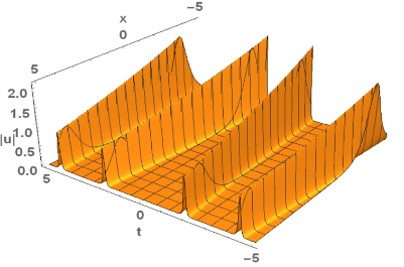
\includegraphics[width=0.4\linewidth]{ss-1.jpg}
		\label{ss-a11}
	}
	\ \
	\subfigure[$\alpha_6(t)=0.5$]{
		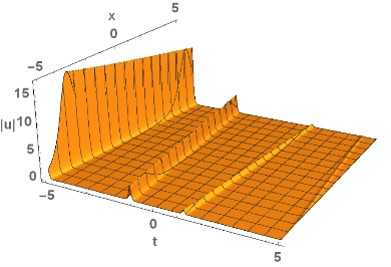
\includegraphics[width=0.4\linewidth]{ss-2.jpg}
		\label{ss-a12}
	}

	\label{a1}

    \centering
	\subfigure[$\alpha_6(t)=t$]{
		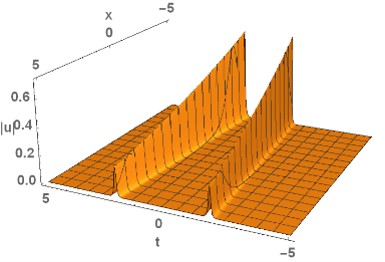
\includegraphics[width=0.4\linewidth]{ss-3.jpg}
		\label{ss-a21}
	}
	\ \
	\subfigure[$\alpha_6(t)=t^3$]{
		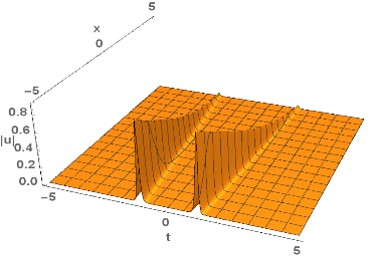
\includegraphics[width=0.4\linewidth]{ss-4.jpg}
		\label{ss-a22}
	}
    \newline
    \newline
    \newline
	\label{a1}

    \centering
	\subfigure[$\alpha_6(t)=cos(t)$]{
		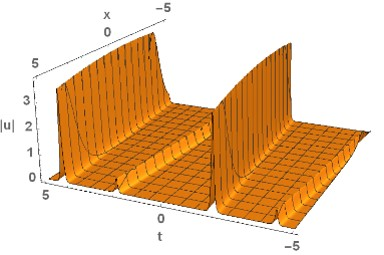
\includegraphics[width=0.4\linewidth]{ss-5.jpg}
		\label{ss-a31}
	}
	\ \
	\subfigure[$\alpha_6(t)=1/t$]{
		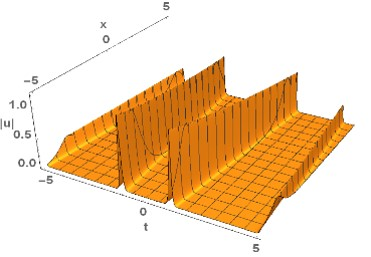
\includegraphics[width=0.4\linewidth]{ss-6.jpg}
		\label{ss-a32}
	}
	\caption{$\alpha_6(t)$的取值不同导致孤立波振幅、波形、传播方向的变化}
	\label{wave-1}
\end{figure}

